\documentclass[a4paper]{article}

\usepackage{hyperref}
%\hypersetup{
%colorlinks=false,              % bool: Liens colorés
%pdfborder={0 0 0}             % Ne pas encadrer les liens
%}
\usepackage[utf8]{inputenc}  
\usepackage[francais]{babel}  
\usepackage[top=2cm, bottom=2cm, left=2cm, right=2cm]{geometry}
\usepackage{graphicx}
\usepackage[final]{pdfpages} 
\usepackage{rotating}
\usepackage{eurosym}
\usepackage{lscape}
\usepackage{float}
% définir les commandes ici

% s'il y a beaucoup de commandes et de packages à inclure n'h&ésitez pas
% à mettre tout ça dans un fichier include.tex et l'inclure
% \input{include.tex}


\begin{document}

%------------------------------------- Page de titre
\begin{titlepage}
~ 
\vfill
	\begin{center}
		\begin{Huge}
		SOA : Dossier de conception détaillée\\
		\end{Huge} 
\vfill
		\textbf{Hexanome 4211 :} 
		\\Sandra \bsc{Mondain}, Elisa \bsc{Abidh}, 
		\\Gaël \bsc{Motte}, Armand \bsc{Rossius}, 
		\\Rémi \bsc{Fradet}, Nicolas \bsc{Silva}, Julien \bsc{Levesy}\\

\vfill		
		\begin{Large}
		Avril 2011
		\end{Large}
\vfill

	\end{center}
\vfill
\end{titlepage}
%----------------------------------------------------

%--------------------------------- Table des matières
\newpage
\tableofcontents
\newpage
%----------------------------------------------- Plan


\section*{Introduction}
Seconde étape de la démarche Top-Down, nous allons maintenant passer à une conception détaillée ciblée de nos différents services métiers et objets métiers. Cependant, afin d'obtenir un découpage au plus proche des besoins de l'utilisateur, il faut avoir une idée claire de l'interface entre notre système d'information et l'utilisateur final. C'est pour cela que nous allons tout d'abord étudier l'enchaînement des fenêtres, leur spécification détaillée pour enfin définir une liste des services (métiers et objets métiers) et une spécification détaillée des services métiers et services objets métiers.

\section{Diagrammes d'Enchainement des Fenêtres}

\subsection{Diagramme d'enchainement des Fenêtre - Client} 

\begin{figure}[H]
	\begin{center}
		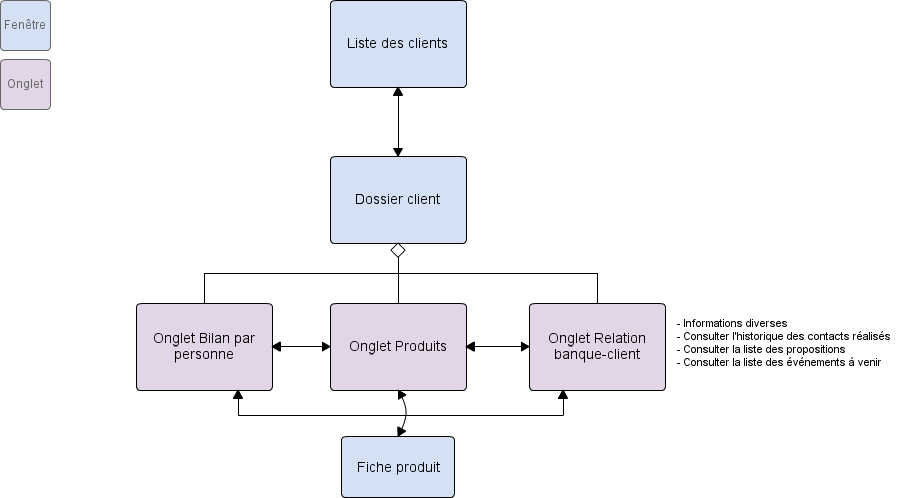
\includegraphics[scale=0.6]{EDF/Client.png}
		\caption{Diagramme d'enchainement des Fenêtre - Client}
	\end{center}
\end{figure}

\subsection{Diagramme d'enchainement des Fenêtre - Contact} 

\begin{figure}[H]
	\begin{center}
		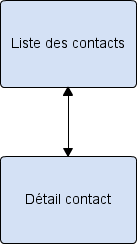
\includegraphics[scale=0.6]{EDF/Contact.png}
		\caption{Diagramme d'enchainement des Fenêtre - Client}
	\end{center}
\end{figure}

\subsection{Diagramme d'enchainement des Fenêtre - Agenda} 

\begin{figure}[H]
	\begin{center}
		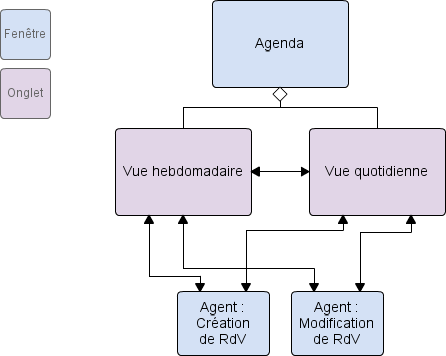
\includegraphics[scale=0.6]{EDF/Agenda.png}
		\caption{Diagramme d'enchainement des Fenêtre - Client}
	\end{center}
\end{figure}
\section{Maquettes de l'IHM} 

	\subsection{Client}
	
		\subsubsection{Liste des clients}
		Cette fenêtre permet de consulter la liste des clients de l'agence et d'effectuer des recherches dans cette liste. Au double-clic sur une ligne, une fenêtre contenant le dossier client correspondant s'ouvre. \\
		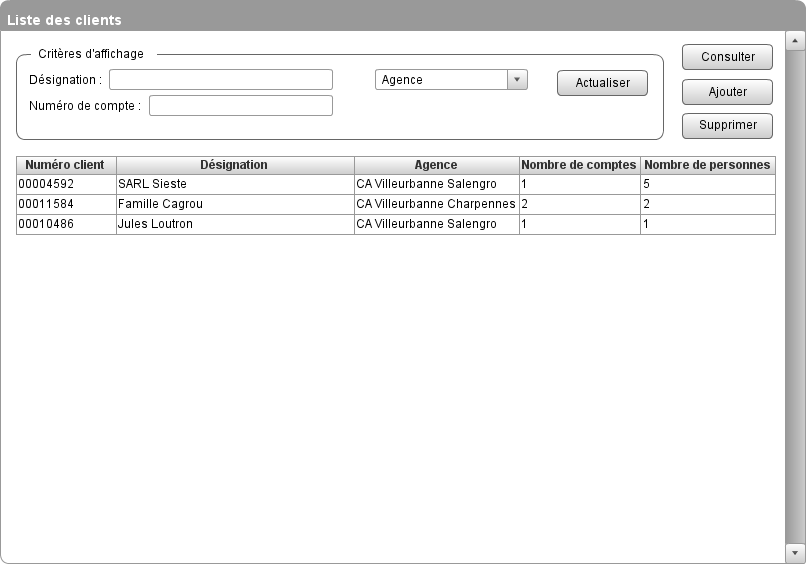
\includegraphics[width=\linewidth]{IHM/Liste_Clients.png}
		
		\newpage		
		
		\subsubsection{Dossier client}
		Lorsque l'on ouvre un dossier client, on accède à ses informations générales (situées en haut de la page). La page contient également 3 onglets : bilan par personne, produits et relation banque-client. Par défaut le premier onglet est sélectionné. \\
		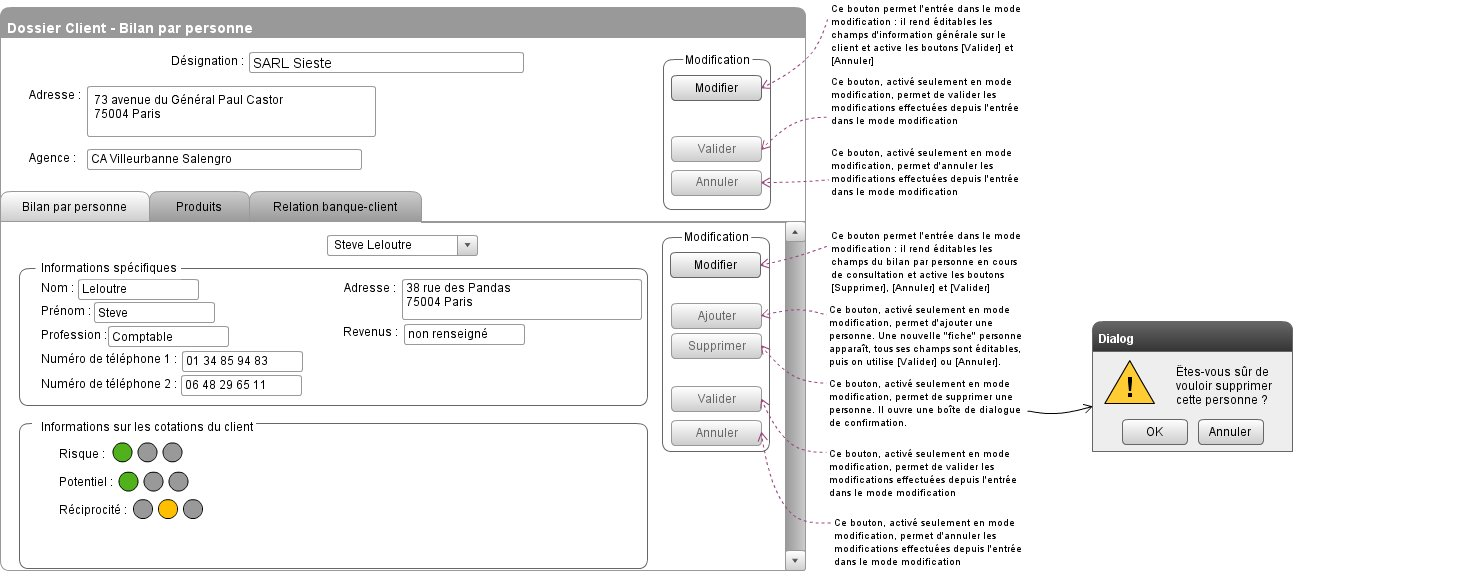
\includegraphics[scale=0.45, angle=90]{IHM/IHMclient1.jpg}
		
		\paragraph*{}
		Ce schéma montre le deuxième onglet. \\
		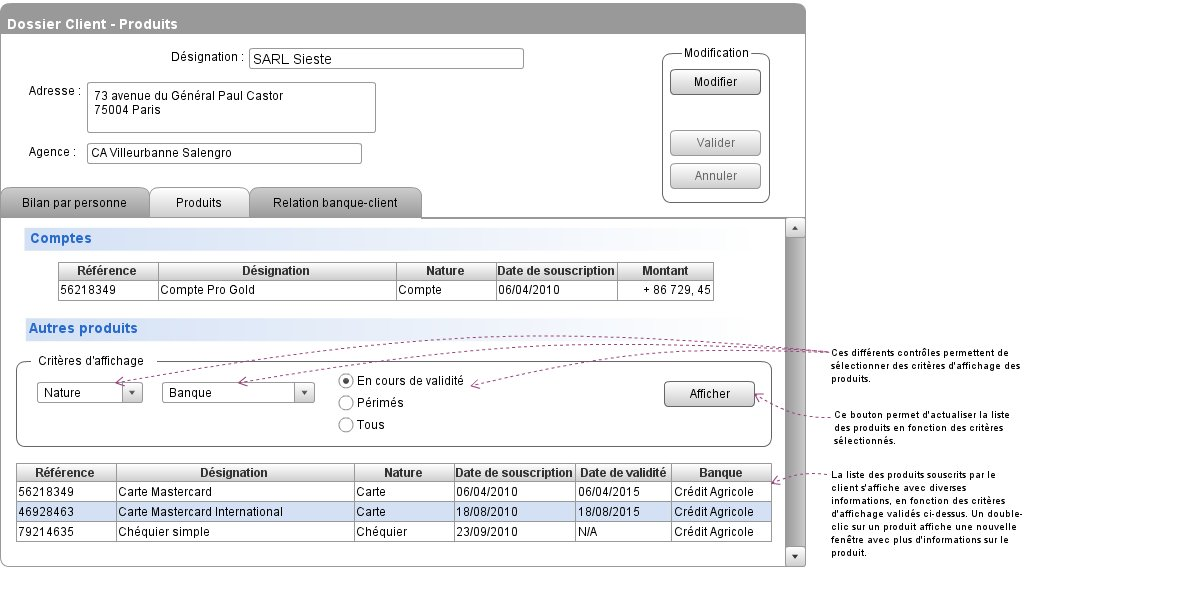
\includegraphics[width=\linewidth]{IHM/IHMclient2.jpg}
		
		\paragraph*{}
		Ces 4 schémas montrent le troisième onglet, qui contient un menu avec 4 options. \\
		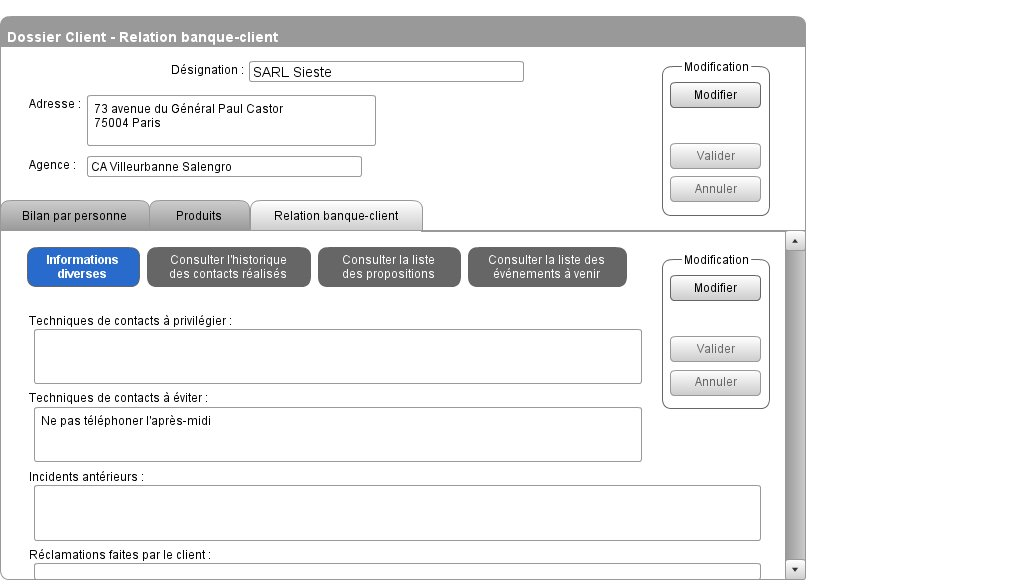
\includegraphics[width=\linewidth]{IHM/IHMclient3.jpg} \\
		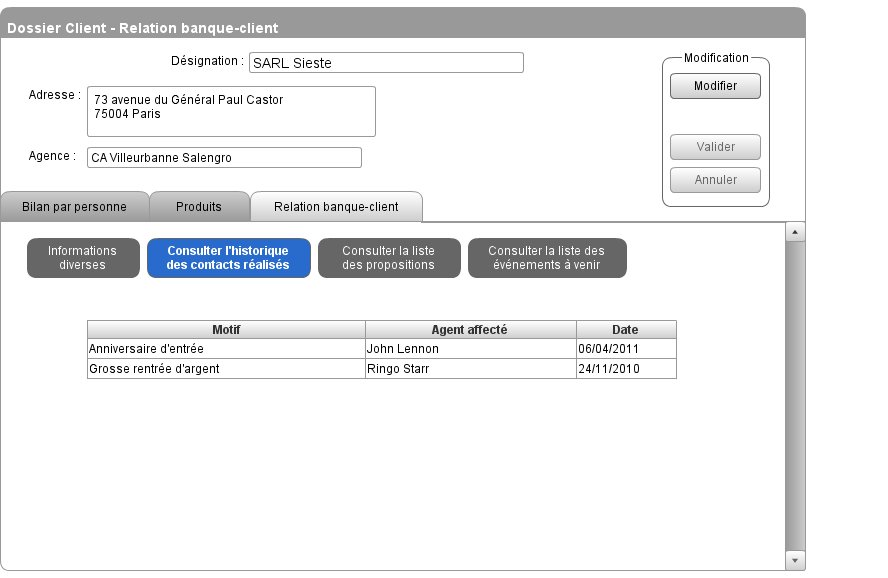
\includegraphics[width=\linewidth]{IHM/IHMclient4.jpg} \\
		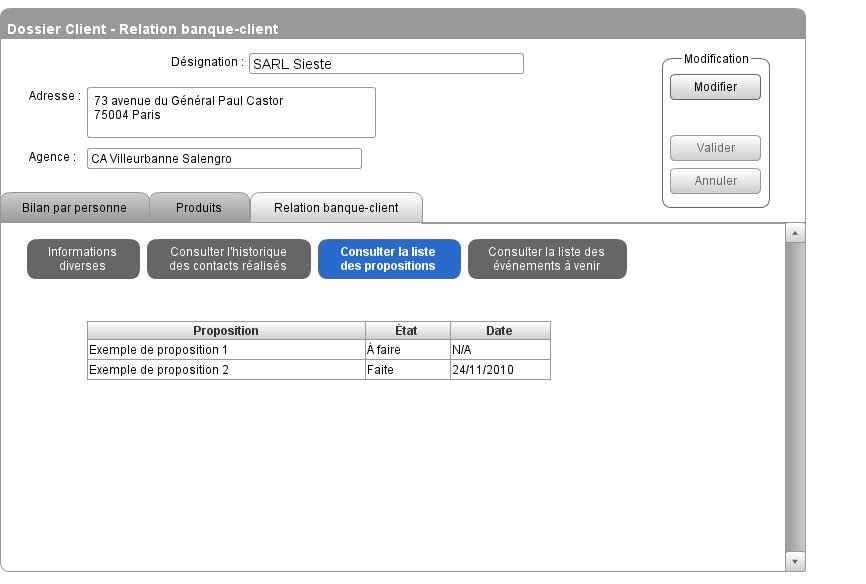
\includegraphics[width=\linewidth]{IHM/IHMclient5.jpg} \\
		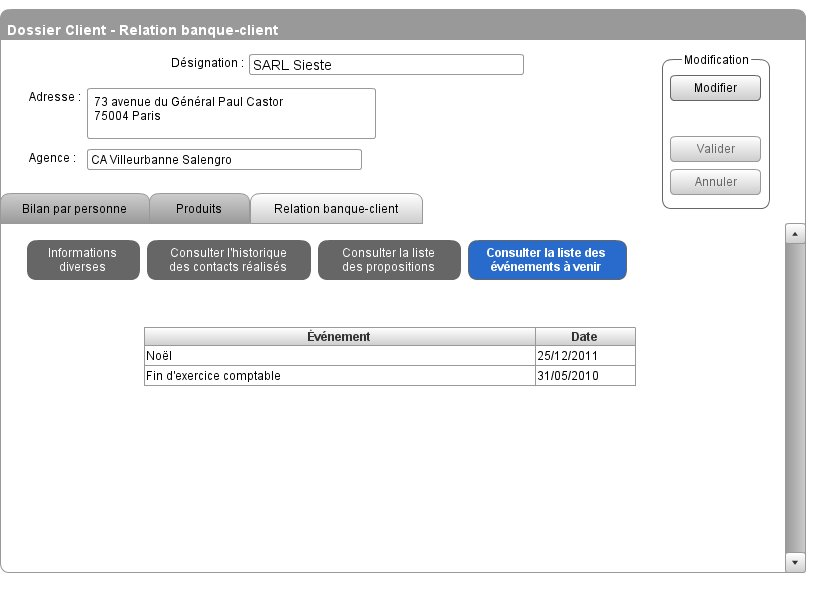
\includegraphics[width=\linewidth]{IHM/IHMclient6.jpg} 
		
	\newpage
		
	\subsection{Contact}
	
		\subsubsection{Liste des contacts}
		Cette fenêtre permet de consulter la liste des contacts de l'agence et d'effectuer des recherches dans cette liste. Au double-clic sur une ligne, une fenêtre contenant les détails du contact correspondant s'ouvre. \\
		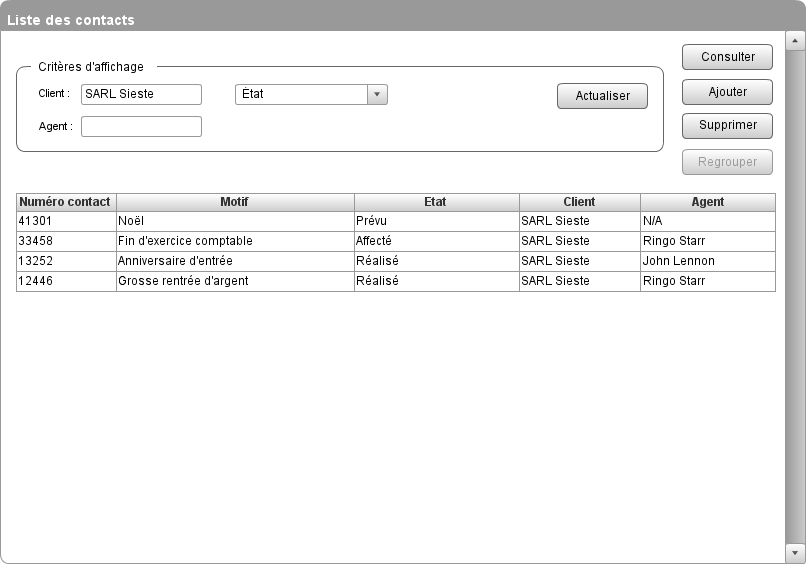
\includegraphics[width=\linewidth]{IHM/Liste_Contacts.png}
		
		\subsubsection{Détail d'un contact}
		Cette fenêtre permet de consulter les détails d'un contact. \\
		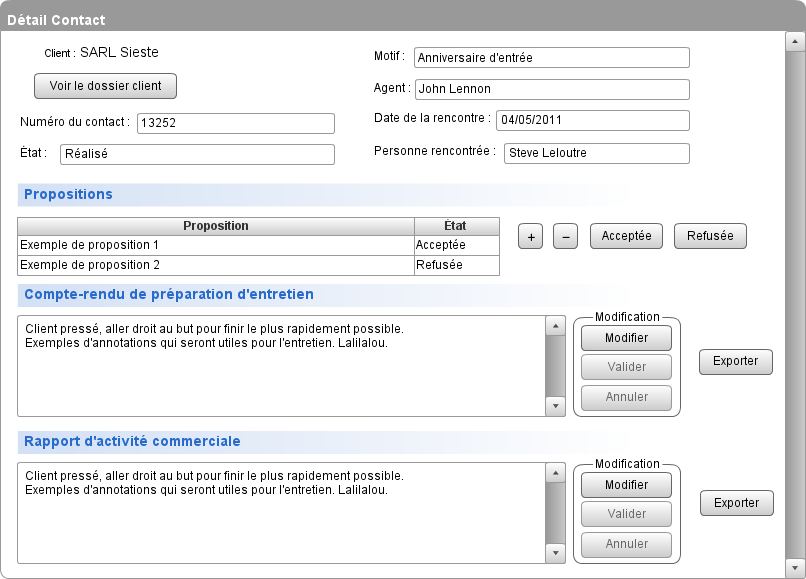
\includegraphics[width=\linewidth]{IHM/Detail_Contact.png}
		
		\newpage
		
	\subsection{Agenda}
		Cette fenêtre permet de consulter l'agenda des agents de l'agence, de créer des plages agenda, de prendre des rendez-vous, de les modifier ou les annuler. \\
		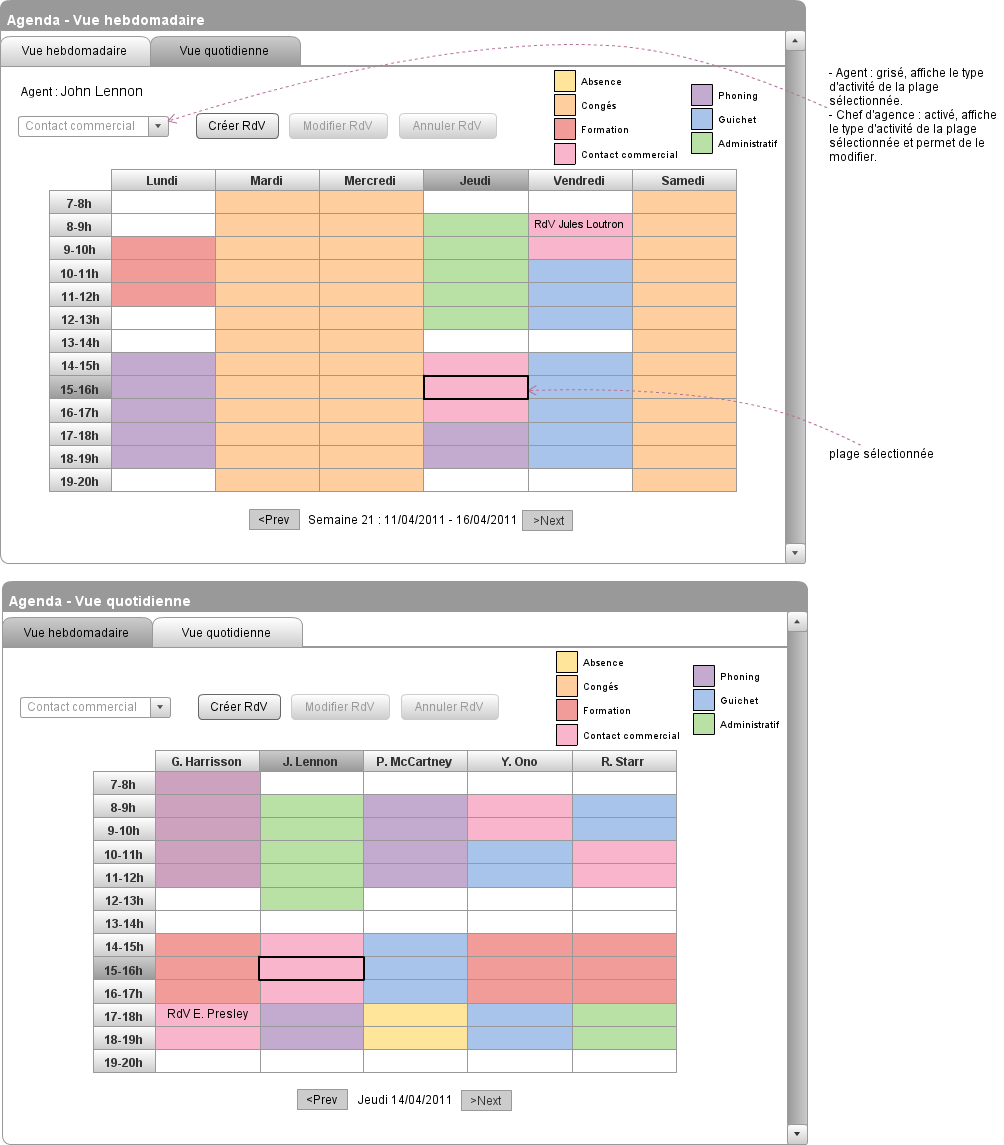
\includegraphics[width=\linewidth]{IHM/Agenda.png}
		
		\newpage
\section{Listes des services}
\subsection{IHM Client}
\subsubsection*{Informations générales}
\begin{itemize}
\item ConsulterInfosClient
\item ModifierInfosClient
\end{itemize}
\subsubsection*{Bilan par personne}
\begin{itemize}
\item ConsulterBilan 
\item ModifierBilan 
\item AjouterPersonne 
\item SupprimerPersonne
\end{itemize}
\subsubsection*{Produit}
\begin{itemize}
\item ConsulterComptesClient 
\item AfficherProduits 
\item SelectionnerProduit 
\item ConsulterFicheProduit
\end{itemize}

\subsubsection*{Relation banque client}
\begin{itemize}
\item ConsulterInfos
\item ConsulterHistoriqueContacts  
\item ConsulterPropositions 
\item ConsulterEvénements 

\end{itemize}

\section{Spécification des services métier}
\subsection{UC1 : Générer contact}
\subsubsection{SM : GenererMotifsContacts}
\begin{itemize}
	\item SOM invoqués : 
	\begin{itemize}
		\item GetEvenementsCaptes [Bloc Evenement]
		\item GenererMotif [Bloc Evenement]
		\item GenererContactPrevu [Bloc Contact]
	\end{itemize}
	\item E : aucun
	\item S : aucune
	\item Procédure : 
	\begin{itemize}
		\item Récupération des évènements captés : GetEvenementsCaptes
		\item Pour chacun des évènement
		\item Génération d’un motif pour chacun des évènements : GenererMotif
		\item Affecter le motif à l’évènement, créant ainsi un nouveau contact prévu : GenererContactPrevu
	\end{itemize}.
\end{itemize}



\subsection{UC2 : Répartition des contacts commerciaux}
\subsubsection{SM : GetContactsPrevus}
\begin{itemize}
	\item SOM invoqués : 
	\begin{itemize}
		\item GetClientsConcernes [Bloc Client]
		\item GetContactsPrevus [Bloc Contact]
	\end{itemize}
	\item E : idAgence
	\item S : Liste de Contacts : idContact, motif, état du contact, Client concerné (nom)
	\item Procédure : 
	\begin{itemize}
		\item Récupération les clients de l’agence : GetClientsConcernes 
		\item Récupération de tous les contacts prévus, pour les clients de l’agence : GetContactsPrevus
	\end{itemize}.
\end{itemize}

\subsubsection{SM : AffecterAgent}
\begin{itemize}
	\item SOM invoqués : 
	\begin{itemize}
		\item AffecterAgent [Bloc Contact]
		\item MAJPotentielMensuel [Bloc Structure]
	\end{itemize}
	\item E : idContact, idAgent
	\item S : aucune
	\item Procédure : 
	\begin{itemize}
		\item Association d’un agent à un contact : AffecterAgent
		\item Calcul du nouveau potentiel mensuel de l’agent concerné par cette affectation : MAJPotentielMensuel
	\end{itemize}.
\end{itemize}




\subsection{UC3 : Suivi de l’action commerciale}

\subsubsection{SM : GetContactByAgent}
\begin{itemize}
	\item SOM invoqués : 
	\begin{itemize}
		\item GetContactByAgent [Bloc Contact]
		\item GetInfoClient [Bloc Client]
		\item GetPersonnel [Bloc Personne]
	\end{itemize}
	\item E : liste d’idContact, 
	\item S : Liste de Contacts : idContact, motif, état du contact, Client concerné (nom)
	\item Procédure : 
	\begin{itemize}
		\item Récupère tous les contacts affectés à un agent : GetContactByAgent
		\item Récupère les information de tous les clients concernés par ces contacts : GetInfoClient
		\item Récupère les informations concernant les personnes référentes des clients concernés : GetPersonnel
	\end{itemize}.
\end{itemize}



\subsection{UC4 : Gestion de la liste des contacts clients}

\subsubsection{SM : GetContactByAgent}
idem UC3 : GetContactByAgent

\subsubsection{SM : CreateGroupContact}
\begin{itemize}
	\item SOM invoqués : 
	\begin{itemize}
		\item CreateGroupContact [Bloc Contact]
	\end{itemize}
	\item E : liste d’idContact
	\item S : validation du SM
	\item Procédure : 
	\begin{itemize}
		\item Crée un groupe de contacts unissant tous les contacts dont les identifiants sont passés en paramètre : CreateGroupContact
	\end{itemize}.
\end{itemize}

\subsubsection{SM : CancelContact}
\begin{itemize}
	\item SOM invoqués : 
	\begin{itemize}
		\item CancelContact [Bloc Contact]
		\item SetContact [Bloc Contact]
	\end{itemize}
	\item E : idContact, motif
	\item S : validation du SM
	\item Procédure : 
	\begin{itemize}
		\item Annulation du Contact, avec affectation d’un motif d’annulation : CancelContact
	\end{itemize}.
\end{itemize}



\subsection{UC6 : Plannification des contacts commerciaux}

\subsubsection{SM : CreerContactSpontane}
\begin{itemize}
	\item SOM invoqués : 
	\begin{itemize}
		\item CreerContactSpontane [Bloc Contact]
	\end{itemize}
	\item E : idClient
	\item S : aucun
	\item Procédure : 
	\begin{itemize}
		\item Crée un contact spontané pour un client donné : CreerContactSpontane
	\end{itemize}.
\end{itemize}

\subsubsection{SM : ConsulterContacts}
\begin{itemize}
	\item SOM invoqués : 
	\begin{itemize}
		\item GetContactByAgent [Bloc Contact]
	\end{itemize}
	\item E : idAgent
	\item S : Liste d’idContact, motif du contact, état
	\item Procédure : 
	\begin{itemize}
		\item Retourne les informations concernant les contacts d'un agent : GetContactByAgent
	\end{itemize}.
\end{itemize}

\subsubsection{SM : CreerRDV}
\begin{itemize}
	\item SOM invoqués : 
	\begin{itemize}
		\item PrendreRDV [Bloc Contact]
		\item GetDetailContact [Agenda]
	\end{itemize}
	\item E : idAgent, idContact, idClient, plageCible
	\item S : aucune
	\item Procédure : 
	\begin{itemize}
		\item Fait passer l’état du contact de affecté à rendez-vous pris
		\item Obtenir les détails du contact
	\end{itemize}.
\end{itemize}



\subsection{UC8 : Préparation d’entretien par un agent}
\subsubsection{SM : ajouterPropositions}
\begin{itemize}
	\item SOM invoqués :
	\begin{itemize}
		\item ajouterProposition
	\end{itemize}
	\item E : liste id\_offres, id\_contact
	\item S : aucun
	\item Procédure :
	\begin{itemize}
		\item Ajoute les propositions au contact : ajouterPropositions
	\end{itemize}.
\end{itemize}

\subsubsection{SM : sauvergarderCR}
\begin{itemize}
	\item SOM invoqués :
	\begin{itemize}
		\item sauvergarderCR
	\end{itemize}
	\item E : id\_contact, texte
	\item S : aucun
	\item Procédure :
	\begin{itemize}
		\item Crée un CR pour le contact : sauvegarderCR
		\item Fait passer le contact à l’état “Préparé” : sauvegarderCR
	\end{itemize}.
\end{itemize}



\subsection{UC9 : Conduite de l’entretien par l’agent}
\subsubsection{SM : sauvergarderRapportActivite}
\begin{itemize}
	\item SOM invoqués :
	\begin{itemize}
		\item sauvergarderRapportActivite
	\end{itemize}
	\item E : id\_contact, texte
	\item S : aucun
	\item Procédure :
	\begin{itemize}
		\item Crée un rapport d’activité pour le contact :
	sauvegarderRapportActivite
		\item Fait passer le contact à l’état “Préparé” : sauvegarderRapportActivite
	\end{itemize}.
\end{itemize}

\subsubsection{SM : accepterProposition}
\begin{itemize}
	\item SOM invoqués :
	\begin{itemize}
		\item accepterProposition
	\end{itemize}
	\item E : id\_contact, id\_proposition
	\item S : aucun
	\item Procédure :
	\begin{itemize}
		\item Accepte la proposition : accepterProposition
	\end{itemize}.
\end{itemize}

\subsubsection{SM : refuserProposition}
\begin{itemize}
	\item SOM invoqués :
	\begin{itemize}
		\item refuserProposition
	\end{itemize}
	\item E : id\_contact, id\_proposition
	\item S : aucun
	\item Procédure :
	\begin{itemize}
		\item Accepte la proposition : refuserProposition
	\end{itemize}.
\end{itemize}

\subsubsection{SM : getPreparation}
\begin{itemize}
	\item SOM invoqués :
	\begin{itemize}
		\item getCRPreparation
		\item getPropositions
		\item getOffre
	\end{itemize}
	\item E : id\_contact
	\item S : CRPréparation, liste propositions(id\_proposition, id\_offre, nom de l’offre)
	\item Procédure :
	\begin{itemize}
		\item Récupère le CR de préparation : getCRPreparation
		\item Récupère les propositions : getPropositions
		\item Récupère le nom des chaque proposition : getOffre
	\end{itemize}.
\end{itemize}



\section{Spécification des services objet-métier}
\subsection{UC1 : Générer contact}
\subsubsection{SOM : GenererContactPrevu}
	\begin{itemize}
		\item E : idEvenement, motif, idClient
		\item S : idMotif
		\item Entité/Classe : Contact : ContactPrevu-MotifContact-Traiter
		\item Rôle : Génère les contact en fonction des évènement-motif-client réalisés
	précédemment.
	\end{itemize}



\subsection{UC2 : Répartition des contacts commerciaux}
\subsubsection{SOM : GetContactPrevu}
	\begin{itemize}
		\item E : Liste d’idClient
		\item S : Liste de Contact : idContact, date de rdv, état du contact, motif...
		\item Entité/Classe : Contact : ContactPrevu-Concerner-Motif
		\item Rôle : Récupère les informations sur les contacts attribués aux clients passés en
	paramètre (les clients de l’agence).
	\end{itemize}

\subsubsection{SOM : AffecterAgent}
	\begin{itemize}
		\item E : idAgent, idContact
		\item S : aucune
		\item Entité/Classe : Contact : Concerner
		\item Rôle : Insérer dans l’entité “Concerner” une association Agent-Contact
	\end{itemize}



\subsection{UC3 : Suivi de l’action commerciale}
\subsubsection{SOM : GetContactByAgent}
	\begin{itemize}
		\item E : idAgent
		\item S : Liste d’idContact, motif, etat, dates changements états, date des rdv associés
		\item Entité/Classe : Contact : ContactPrevu, Concerner, MotifContact, Traiter
		\item Rôle : Récupère les informations sur les contacts prévus pour un agent donné
	(passé en paramètre).
	\end{itemize}



\subsection{UC4 : Gestion de la liste des contacts clients}
\subsubsection{SOM : GetContactByAgent}
	\begin{itemize}
		\item E : idAgent
		\item S : Liste d’idContact, motif, etat, dates changements états, date des rdv associés
		\item Entité/Classe : Contact : ContactPrevu, Concerner, MotifContact, Traiter
		\item Rôle : Récupère les informations sur les contacts prévus pour un agent donné
	(passé en paramètre).
	\end{itemize}

\subsubsection{SOM : CreateGroupContact}
	\begin{itemize}
		\item E : List d’idContact
		\item S : booléen de validation d’opération
		\item Entité/Classe : Contact : ContactPrevu
		\item Rôle : Groupe plusieurs contacts en un seul contact prévu.
	\end{itemize}

\subsubsection{SOM : CancelContact}
	\begin{itemize}
		\item E : idContact, Motif
		\item S : booléen de validation d’opération
		\item Entité/Classe : Contact : ContactPrevu
		\item Rôle : Modifie l’état d’un contact en le passant “Annulé”.
	\end{itemize}



\subsection{UC5 : Planification de l’activité de l’agence du mois suivant}
Pas de SOM du bloc contact



\subsection{UC6 : Planification des contact commerciaux}
\subsubsection{SOM : GetContactByAgent}
	\begin{itemize}
		\item E : id\_agent
		\item S : liste contacts(id\_contact, date du contact, motif du contact...)
		\item Entité/Classe : Contact, Motif de contact
		\item Rôle : Renvoi la liste des contacts pour un agent donné
	\end{itemize}

\subsubsection{SOM : prendreRDV}
	\begin{itemize}
		\item E : id\_contact
		\item S : aucun
		\item Entité/Classe : Contact
		\item Rôle : Fait passer l’état du contact de affecté à rendez-vous pris
	\end{itemize}

\subsubsection{SOM : creerContactSpontane}
	\begin{itemize}
		\item E : id\_client
		\item S : aucun
		\item Entité/Classe : Contact
		\item Rôle : Crée un contact dont l’état est Réalisé
	\end{itemize}



\subsection{UC7 : Consultation des agendas}
Pas de SOM du bloc contact



\subsection{UC8 : Préparation d’entretien par un agent}
\subsubsection{SOM : ajouterPropositions}
	\begin{itemize}
		\item E : liste id\_offres, id\_contact
		\item S : aucun
		\item Entité/Classe : Contact Réalisé, Proposition commerciale
		\item Rôle : Crée une proposition commerciale au contact pour chacune des offres de la
	liste.
	\end{itemize}

\subsubsection{SOM : sauvegarderCR}
	\begin{itemize}
		\item E : idContact, texte
		\item S : aucun
		\item Entité/Classe : Contact
		\item Rôle : Crée le compte rendu de préparation pour le contact., Fait passer le contact
	de l’état Rendez-vous Pris à préparé.
	\end{itemize}



\subsection{UC9 : Conduite de l‘entretien par l’agent}
\subsubsection{SOM : getContactState}
	\begin{itemize}
		\item E : id\_contact
		\item S : état du contact (prévu, réalisé, …)
		\item Entité/Classe : Contact
		\item Rôle : Renvoi l’état d’un contact
	\end{itemize}

\subsubsection{SOM : getCRPréparation}
	\begin{itemize}
		\item E : id\_contact
		\item S : CRPréparation
		\item Entité/Classe : Contact
		\item Rôle : Renvoie le CR de préparation de l’entretien (s’il existe)
	\end{itemize}

\subsubsection{SOM : getProposition}
	\begin{itemize}
		\item E : id\_contact
		\item S : liste propositions (id\_proposition, id\_offre, nom de l’offre)
		\item Entité/Classe : Contact, Proposition Commerciale
		\item Rôle : renvoie les propositions commerciales faites à un contact
	\end{itemize}

\subsubsection{SOM : accepterProposition}
	\begin{itemize}
		\item E : id\_proposition, id\_contact
		\item S : aucun
		\item Entité/Classe : Contact, Proposition Commerciale
		\item Rôle : accepte la proposition commerciale
	\end{itemize}

\subsubsection{SOM : refuserProposition}
	\begin{itemize}
		\item E : id\_proposition, id\_contact
		\item S : aucun
		\item Entité/Classe : Contact, Proposition Commerciale
		\item Rôle : refuse la proposition commerciale
	\end{itemize}

\subsubsection{SOM : sauvegarderRapportActivite}
	\begin{itemize}
		\item E : id\_contact, texte
		\item S : aucun
		\item Entité/Classe : Contact
		\item Rôle : Crée le rapport d’activité commerciale pour le contact et fait passer l’état du
	contact à “réalisé”
	\end{itemize}



\subsection{UC10 : Consultation du dossier client}

\subsubsection{SOM :getContact}
	\begin{itemize}
		\item E : id\_contact
		\item S : infos\_contact(nom du contact, motif, …)
		\item Entité/Classe : Contact, Motif de contact
		\item Rôle : Renvoi les informations sur le contact
	\end{itemize}

\subsubsection{SOM : getPropositionCommerciales}
	\begin{itemize}
		\item E : id\_contact
		\item S : liste propositionCommerciales(id\_proposition, id\_offre)
		\item Entité/Classe : Contact, Proposition Commerciale
		\item Rôle : Renvoie le CR de préparation de l’entretien (s’il existe)
	\end{itemize}


\end{document}
